% Standalone export of the report's env-loop figure (fig:e2-env-loop in
% report_latex/chapters/AdaptiveRLMRI.tex) for the presentation deck.
% Build:  presentation/make_envloop.sh   (lualatex -> pdf -> gs -> png)
\documentclass[border=6pt]{standalone}
\usepackage{tikz}
\usepackage{amsmath}
\usetikzlibrary{positioning,arrows.meta,fit,calc,backgrounds,shapes.geometric}

% New brand ImperialBlue (from ic_eee_thesis.cls)
\definecolor{ImperialBlue}{RGB}{0,0,205}

\begin{document}
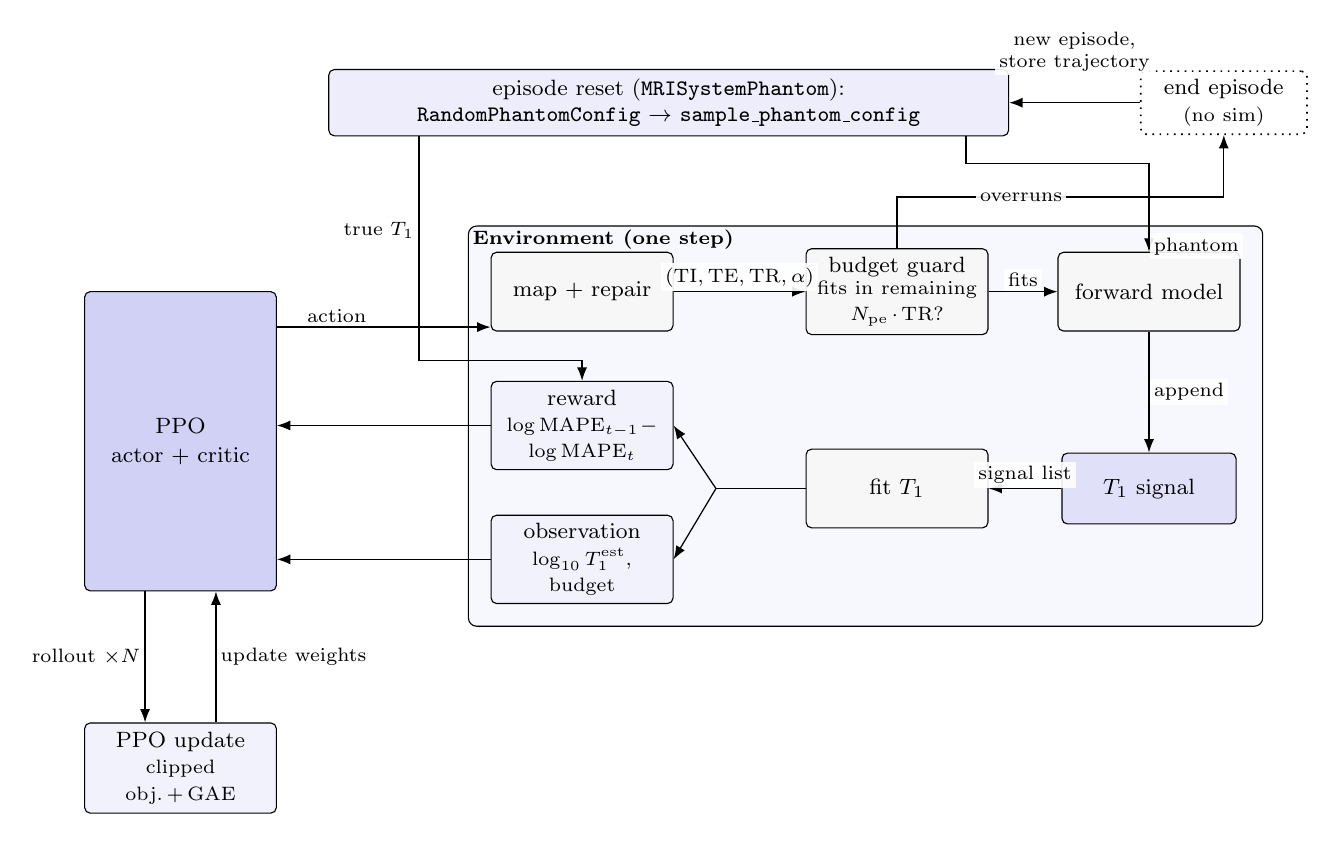
\begin{tikzpicture}[
  font=\footnotesize,
  proc/.style={draw, rounded corners=2pt, align=center, inner xsep=3pt,
    inner ysep=3pt, minimum height=10mm, text width=21mm, fill=black!3},
  state/.style={draw, rounded corners=2pt, align=center, inner xsep=3pt,
    inner ysep=3pt, minimum height=9mm, text width=20mm, fill=ImperialBlue!12},
  io/.style={draw, rounded corners=2pt, align=center, inner xsep=3pt,
    inner ysep=3pt, minimum height=9mm, text width=21mm, fill=ImperialBlue!5},
  endb/.style={draw, dotted, line width=0.6pt, rounded corners=2pt, align=center,
    inner xsep=3pt, inner ysep=3pt, minimum height=8mm, text width=19mm},
  agent/.style={draw, rounded corners=2pt, align=center, fill=ImperialBlue!18,
    text width=22mm, minimum height=38mm},
  reset/.style={draw, rounded corners=2pt, align=center, fill=ImperialBlue!7,
    text width=84mm, minimum height=8mm},
  upd/.style={draw, rounded corners=2pt, align=center, fill=ImperialBlue!5,
    text width=22mm, minimum height=9mm},
  arr/.style={-{Latex[length=1.7mm]}, line width=0.45pt},
  lbl/.style={font=\scriptsize, inner sep=1.5pt, fill=white, fill opacity=0.9,
    text opacity=1},
]
\node[agent] (ppo) at (0,1.0) {PPO\\[1pt] actor $+$ critic};
\node[upd] (update) at (0,-3.15) {PPO update\\ \scriptsize clipped obj.\,$+$\,GAE};

\node[proc] (map)   at (5.1,2.9)  {map $+$ repair};
\node[proc] (guard) at (9.1,2.9)  {budget guard\\ \scriptsize fits in remaining\\ $N_\mathrm{pe}\!\cdot\!\mathrm{TR}$?};
\node[proc] (fwd)   at (12.3,2.9) {forward model};

\node[io] (rew) at (5.1,1.2)  {reward\\ \scriptsize $\log\mathrm{MAPE}_{t-1}\!-\!\log\mathrm{MAPE}_t$};
\node[io] (obs) at (5.1,-0.5) {observation\\ \scriptsize $\log_{10}T_1^{\mathrm{est}}$, budget};

\node[state] (sig) at (12.3,0.4) {$T_1$ signal};
\node[proc]  (fit) at (9.1,0.4)  {fit $T_1$};

\node[reset] (reset) at (6.2,5.3)
  {episode reset (\texttt{MRISystemPhantom}):
   \texttt{RandomPhantomConfig} $\to$ \texttt{sample\_phantom\_config}};
\node[endb] (end) at (13.25,5.3) {end episode\\ \scriptsize (no sim)};

\begin{scope}[on background layer]
\node[draw, rounded corners=3pt, fill=ImperialBlue!3, inner sep=8pt,
      fit=(map)(guard)(fwd)(sig)(fit)(rew)(obs)] (envbox) {};
\node[lbl, anchor=north west, fill=none] at (envbox.north west) {\textbf{Environment (one step)}};
\end{scope}

\coordinate (actionout) at ($(ppo.east)+(0,1.45)$);
\draw[arr] (actionout) -- (map.west|-actionout)
  node[lbl, pos=0.28, above] {action};
\draw[arr] (map) -- (guard) node[lbl, midway, above] {\scriptsize$(\mathrm{TI},\mathrm{TE},\mathrm{TR},\alpha)$};
\draw[arr] (guard) -- (fwd) node[lbl, midway, above] {fits};

\draw[arr] (guard.north) -- ++(0,0.65) -| (end.south)
  node[lbl, pos=0.12, right] {overruns};
\draw[arr] (end.west) -- (reset.east)
  node[lbl, midway, align=center, yshift=6.5mm] {new episode,\\ store trajectory};

\coordinate (phantomout) at ($(reset.south east)+(-0.55,0)$);
\draw[arr] (phantomout) -- ++(0,-0.34) -| (fwd.north)
  node[lbl, pos=0.88, right, yshift=-2mm] {phantom};
\coordinate (t1bus) at ($(envbox.west)+(-0.62,0)$);
\coordinate (t1drop) at ($(rew.north)+(0,0.26)$);
\draw[arr] (reset.south-|t1bus) --
  node[lbl, pos=0.42, left] {true $T_1$}
  (t1bus|-t1drop) -- (t1drop) -- (rew.north);

\draw[arr] (fwd.south) -- (sig.north) node[lbl, midway, right] {append};
\draw[arr] (sig) -- (fit) node[lbl, midway, above] {signal list};
\coordinate (fork) at (6.8,0.4);
\draw (fit.west) -- (fork);
\draw[arr] (fork) -- (rew.east);
\draw[arr] (fork) -- (obs.east);

\draw[arr] (rew.west) -- (ppo.east|-rew);
\draw[arr] (obs.west) -- (ppo.east|-obs);

\draw[arr] ($(ppo.south)+(-0.45,0)$) -- ($(update.north)+(-0.45,0)$)
  node[lbl, midway, left] {rollout $\times N$};
\draw[arr] ($(update.north)+(0.45,0)$) -- ($(ppo.south)+(0.45,0)$)
  node[lbl, midway, right] {update weights};
\end{tikzpicture}
\end{document}
